{\color{rred}\section{Variazione Totale}}
\textcolor{rred}{\rule[5pt]{\textwidth}{1pt}}
Tramite un algoritmo possiamo recuperare immagini sfocate basandoci sulla Variazione totale partendo da una Blurring Point-Spread function di un'immagine. 

La variazione totale è definita dalla seguente formula:                                                                                

\[TV(u) = \sum_i^n{\sum_j^m{\sqrt{||\nabla u(i, j)||_2^2 + \epsilon^2}}}\]

Per calcolare il gradiente dell'immagine $\nabla u$ usiamo la funzione \code{np.gradient} che approssima la derivata per ogni pixel calcolando la differenza tra pixel adiacenti. 

I risultati sono due immagini della stessa dimensione dell'immagine in input, una che rappresenta il valore della derivata orizzontale dx e l'altra della derivata verticale dy. Il gradiente dell'immagine nel punto $(i, j)$ è quindi un vettore di due componenti, uno orizzontale contenuto in dx e uno verticale in dy.
\[x^* = \arg\min_x \frac{1}{2} ||Ax - b||_2^2 + \lambda TV(u)\] 
il cui gradiente $\nabla f$ è dato da: 
\[\nabla f(x) = (A^TAx - A^Tb)  + \lambda \nabla TV(x)\]

{\color{rred}\subsection{Variazione totale delle immagini geometriche:}}
{\color{rred}\subsubsection{Immagine geometrica img2.png}}
\begin{figure}[H]{}
    \centering
    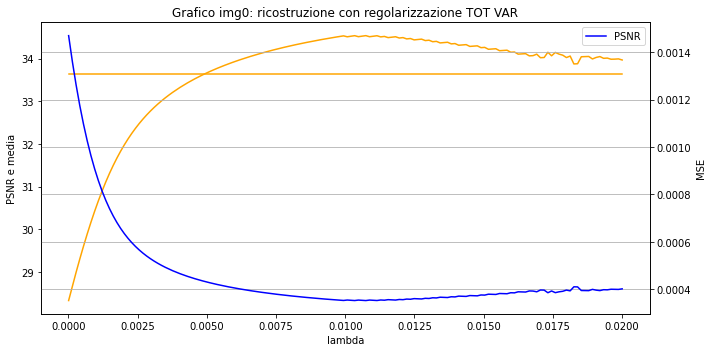
\includegraphics[width=0.5\textwidth]{IMMAGINI_RELAZIONE/grafico2TOTVAR_riserva.png}%
    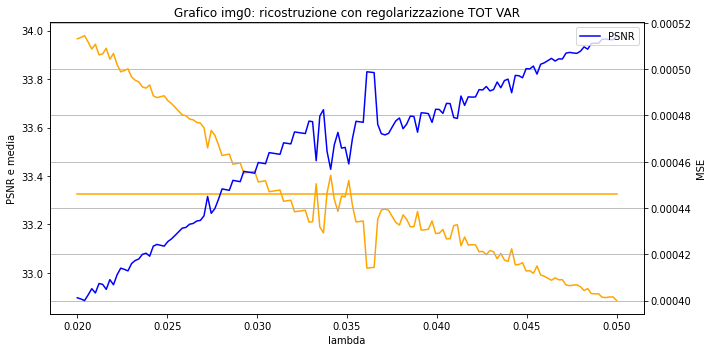
\includegraphics[width=0.5\textwidth]{IMMAGINI_RELAZIONE/proseguimentoGraficoTOTVAR2.png}
    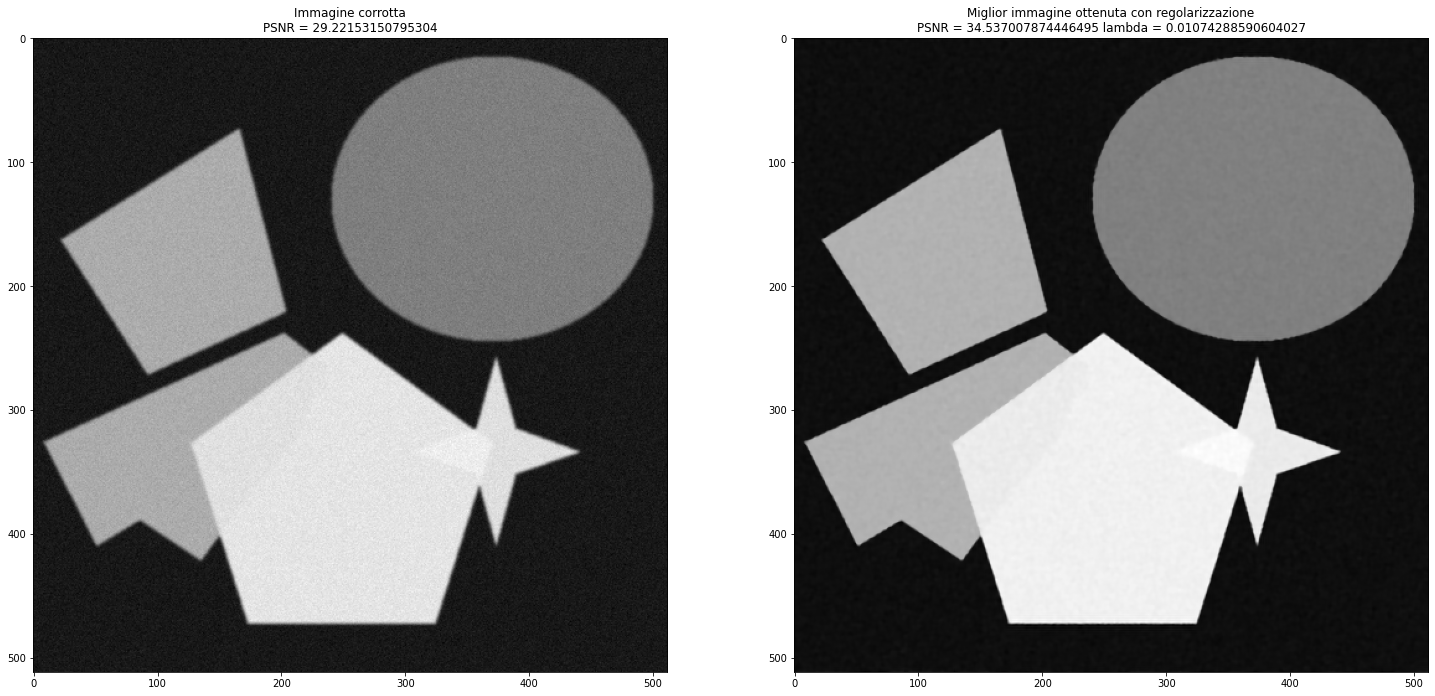
\includegraphics[width=0.8\textwidth]{IMMAGINI_RELAZIONE/ricostruzione2TOTVAR.png}
    \caption{Immagine Corrotta, Immagine Ricostruita}
\end{figure}

{\color{rred}\subsubsection{Immagine geometrica img4.png}}
\begin{figure}[H]{}
    \centering
    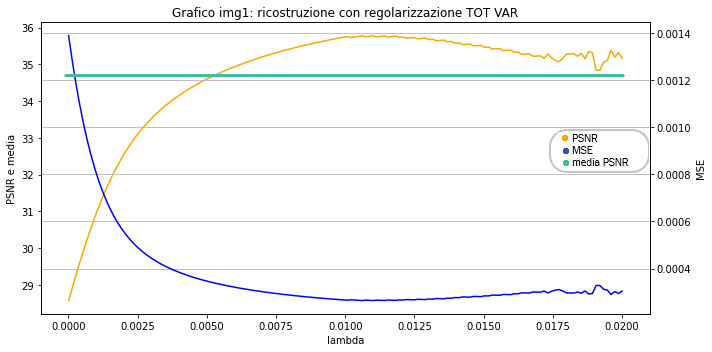
\includegraphics[width=0.5\textwidth]{IMMAGINI_RELAZIONE/grafico4TOTVAR_riserva.png}%
    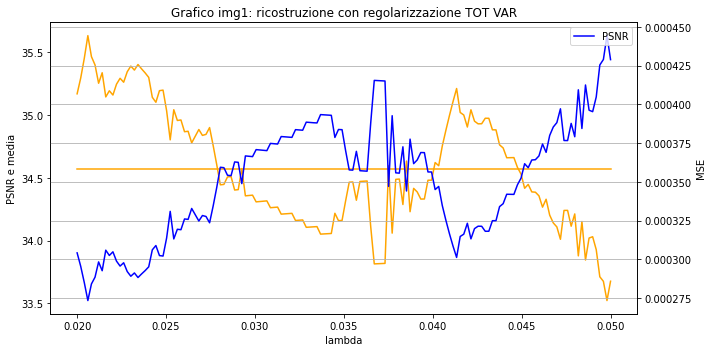
\includegraphics[width=0.5\textwidth]{IMMAGINI_RELAZIONE/proseguimentoGraficoTOTVAR4.png}
    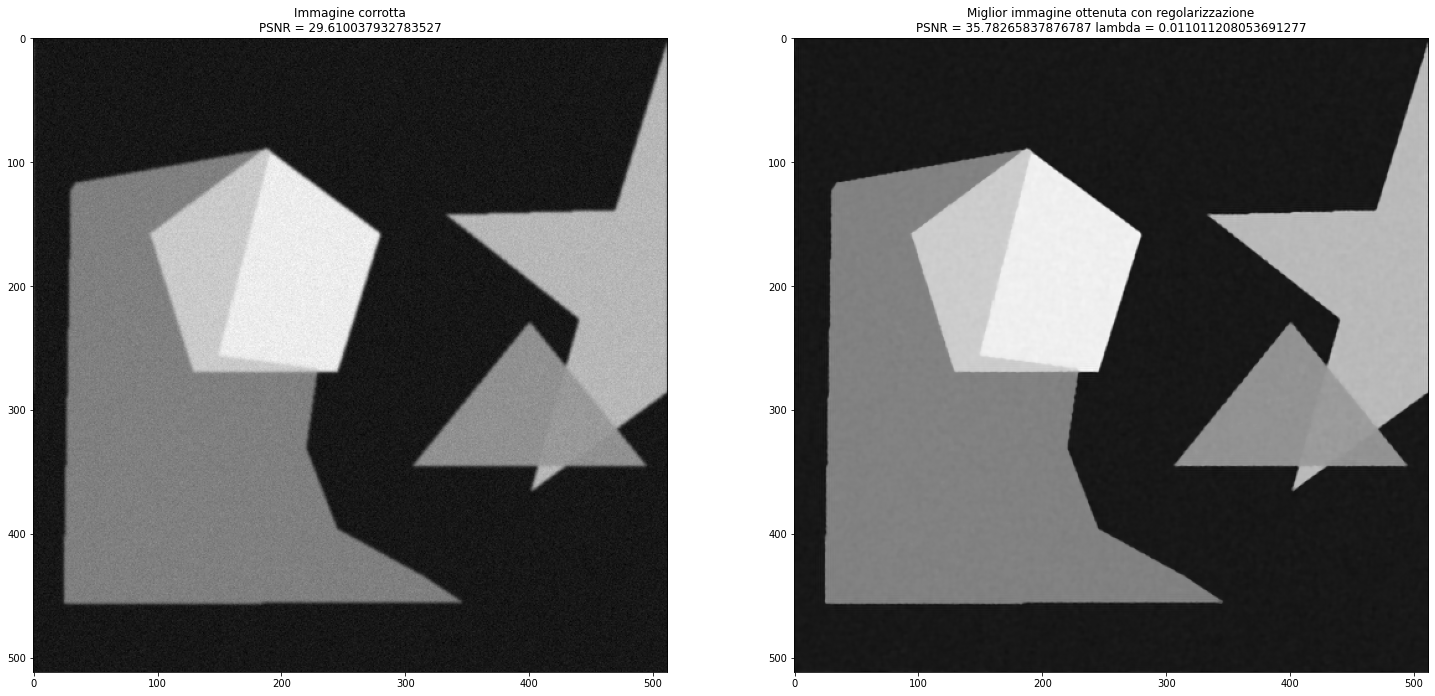
\includegraphics[width=0.8\textwidth]{IMMAGINI_RELAZIONE/ricostruzione4TOTVAR.png}
    \caption{Immagine Corrotta, Immagine Ricostruita}
\end{figure}

{\color{rred}\subsubsection{Immagine geometrica img6.png}}
\begin{figure}[H]{}
    \centering
    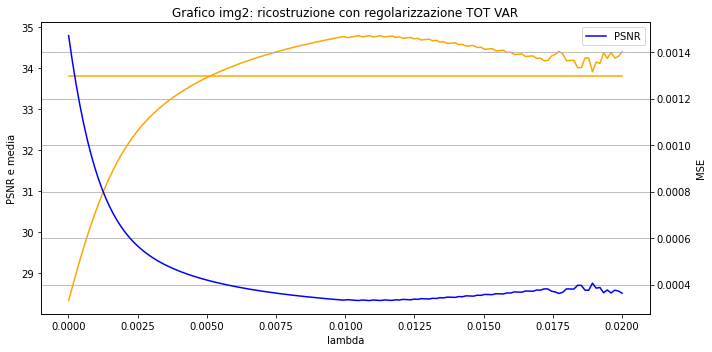
\includegraphics[width=0.5\textwidth]{IMMAGINI_RELAZIONE/grafico6TOTVAR_riserva.png}%
    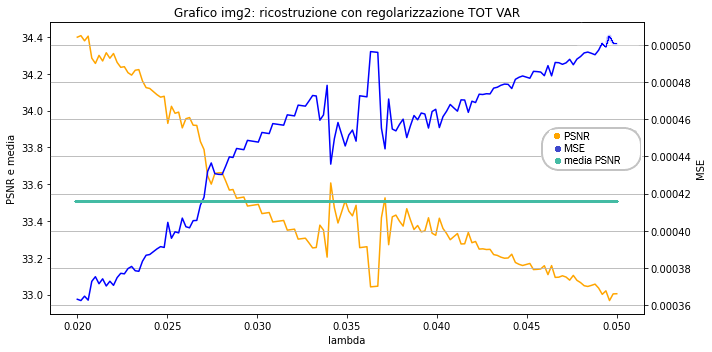
\includegraphics[width=0.5\textwidth]{IMMAGINI_RELAZIONE/proseguimentoGraficoTOTVAR6.png}
    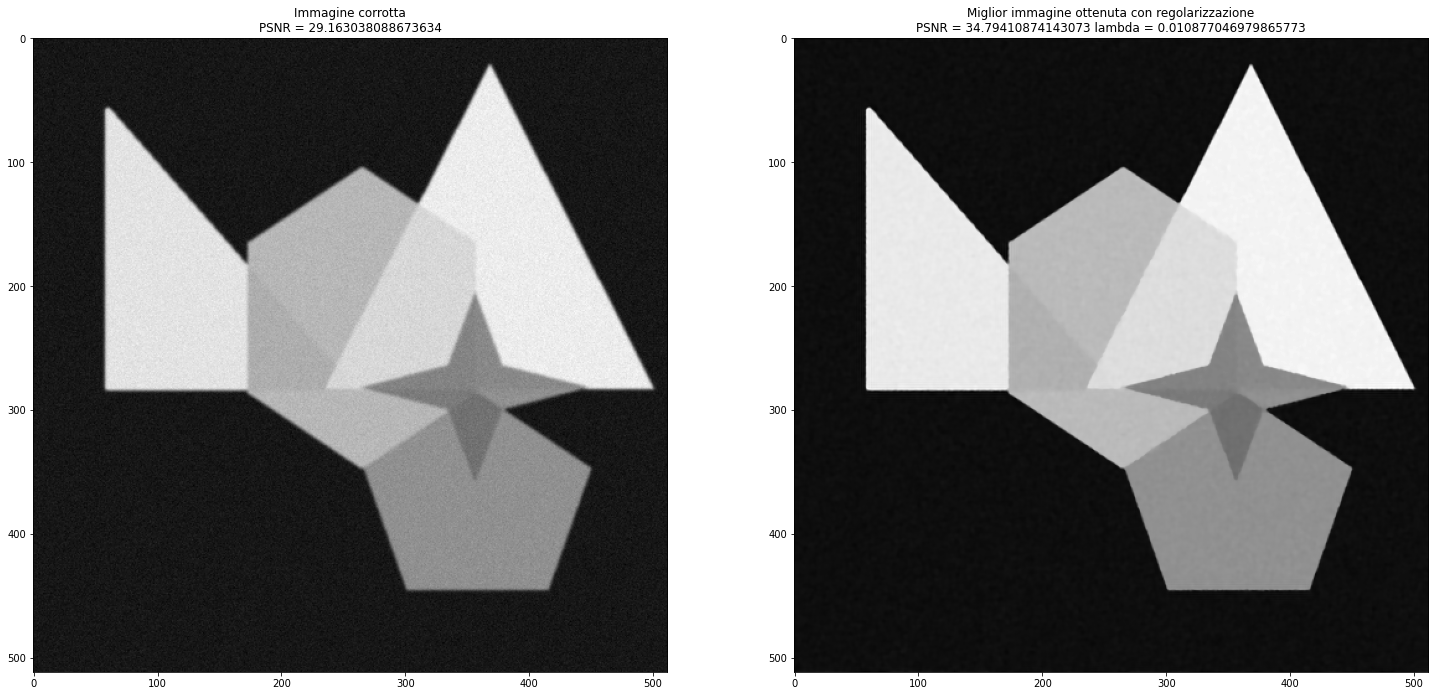
\includegraphics[width=0.8\textwidth]{IMMAGINI_RELAZIONE/ricostruzione6TOTVAR.png}
    \caption{Immagine Corrotta, Immagine Ricostruita}
\end{figure}


{\color{rred}\subsection{Variazione totale dell'immagine ritratto:}}
\begin{figure}[H]{}
    \centering
    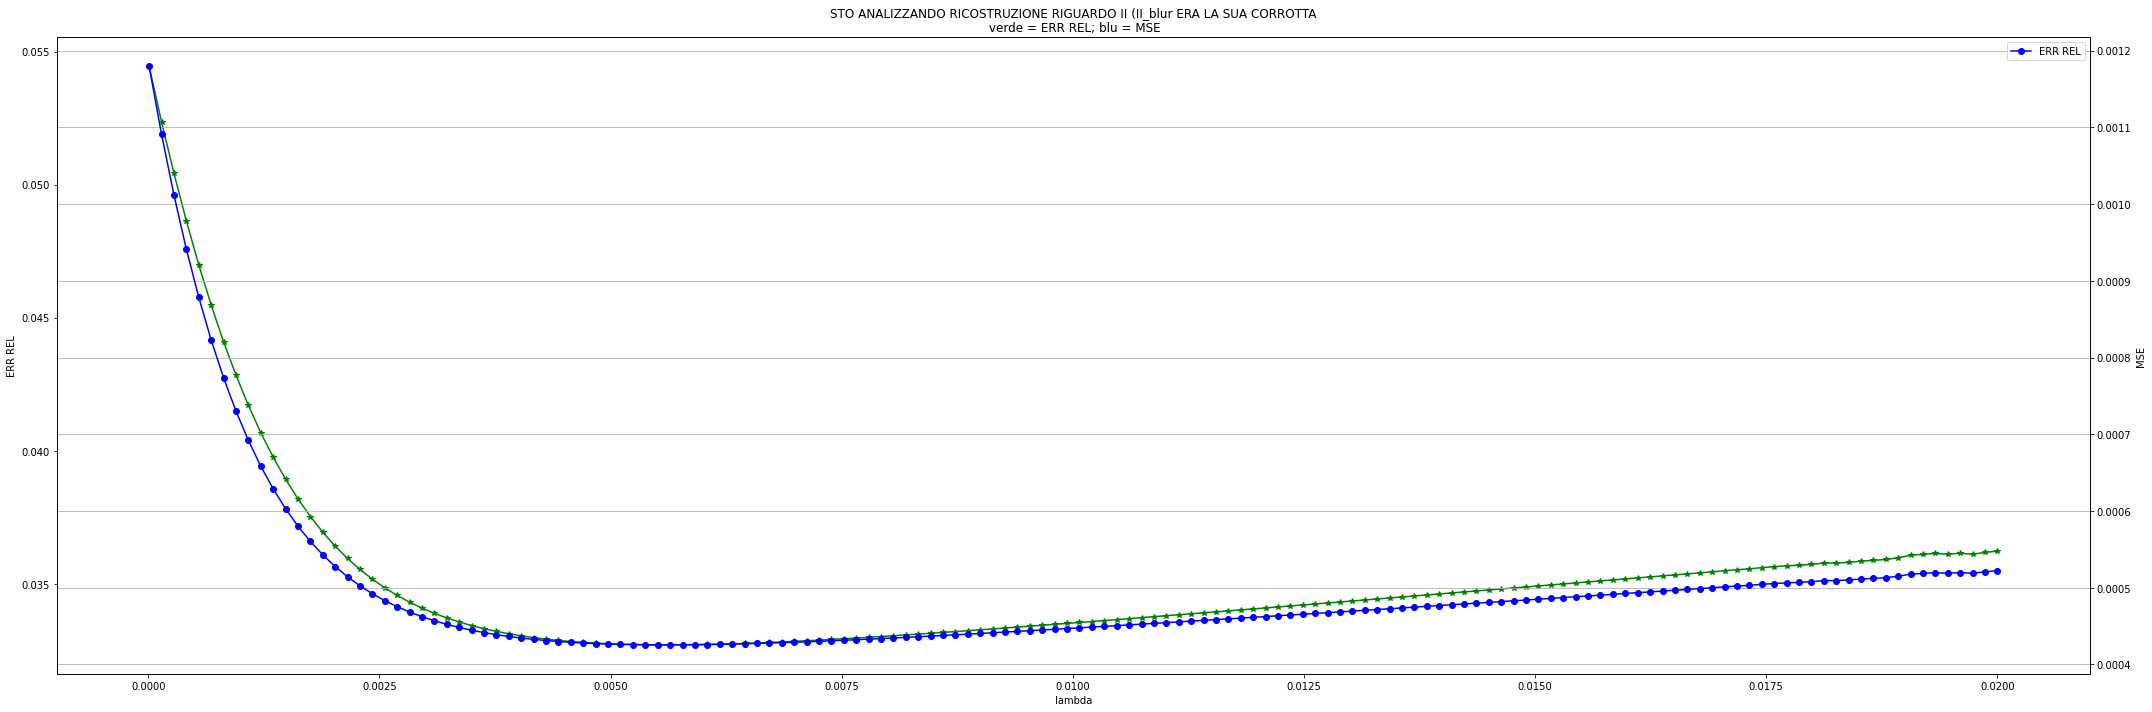
\includegraphics[width=0.8\textwidth]{IMMAGINI_RELAZIONE/graficoPugileTOTVAR_ERRREL&MSE.png}
    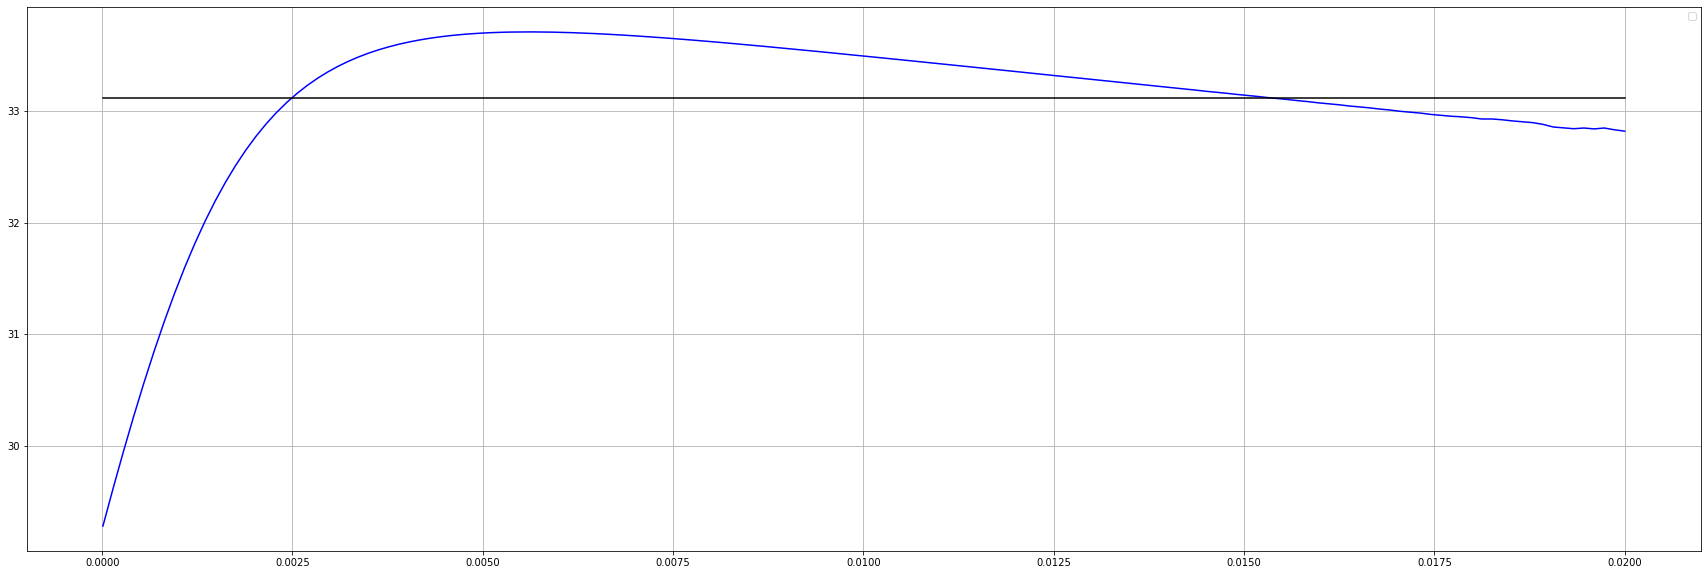
\includegraphics[width=0.8\textwidth]{IMMAGINI_RELAZIONE/graficoPugileTOTVAR_PSNR&suaMedia.png}
    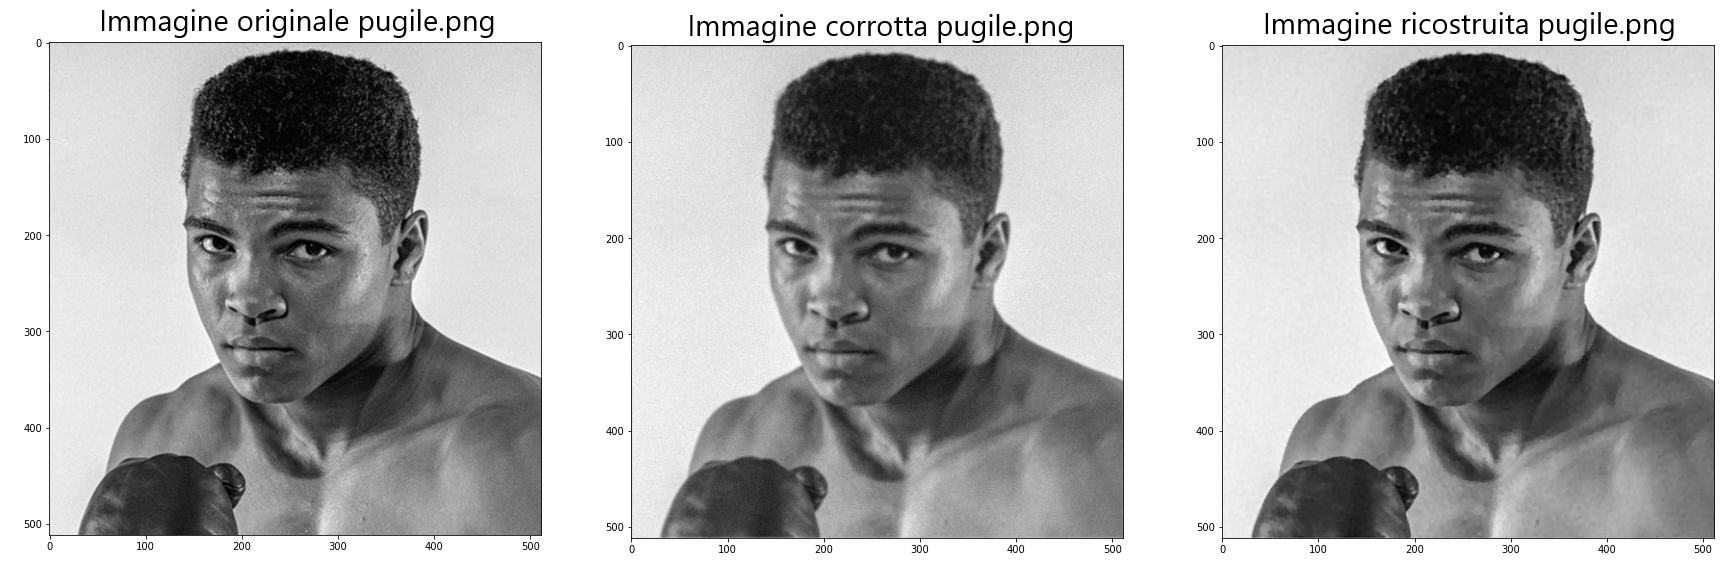
\includegraphics[width=0.8\textwidth]{imgRicostruzione/ricostruzionePugile_TOTVAR_maxPSNR33.70.png}
    \caption{Immagine Originale, Immagine Corrotta, Immagine Ricostruita}
\end{figure}


{\color{rred}\subsection{Variazione totale dell'immagine con testo:}}
\begin{figure}[H]{}
    \centering
    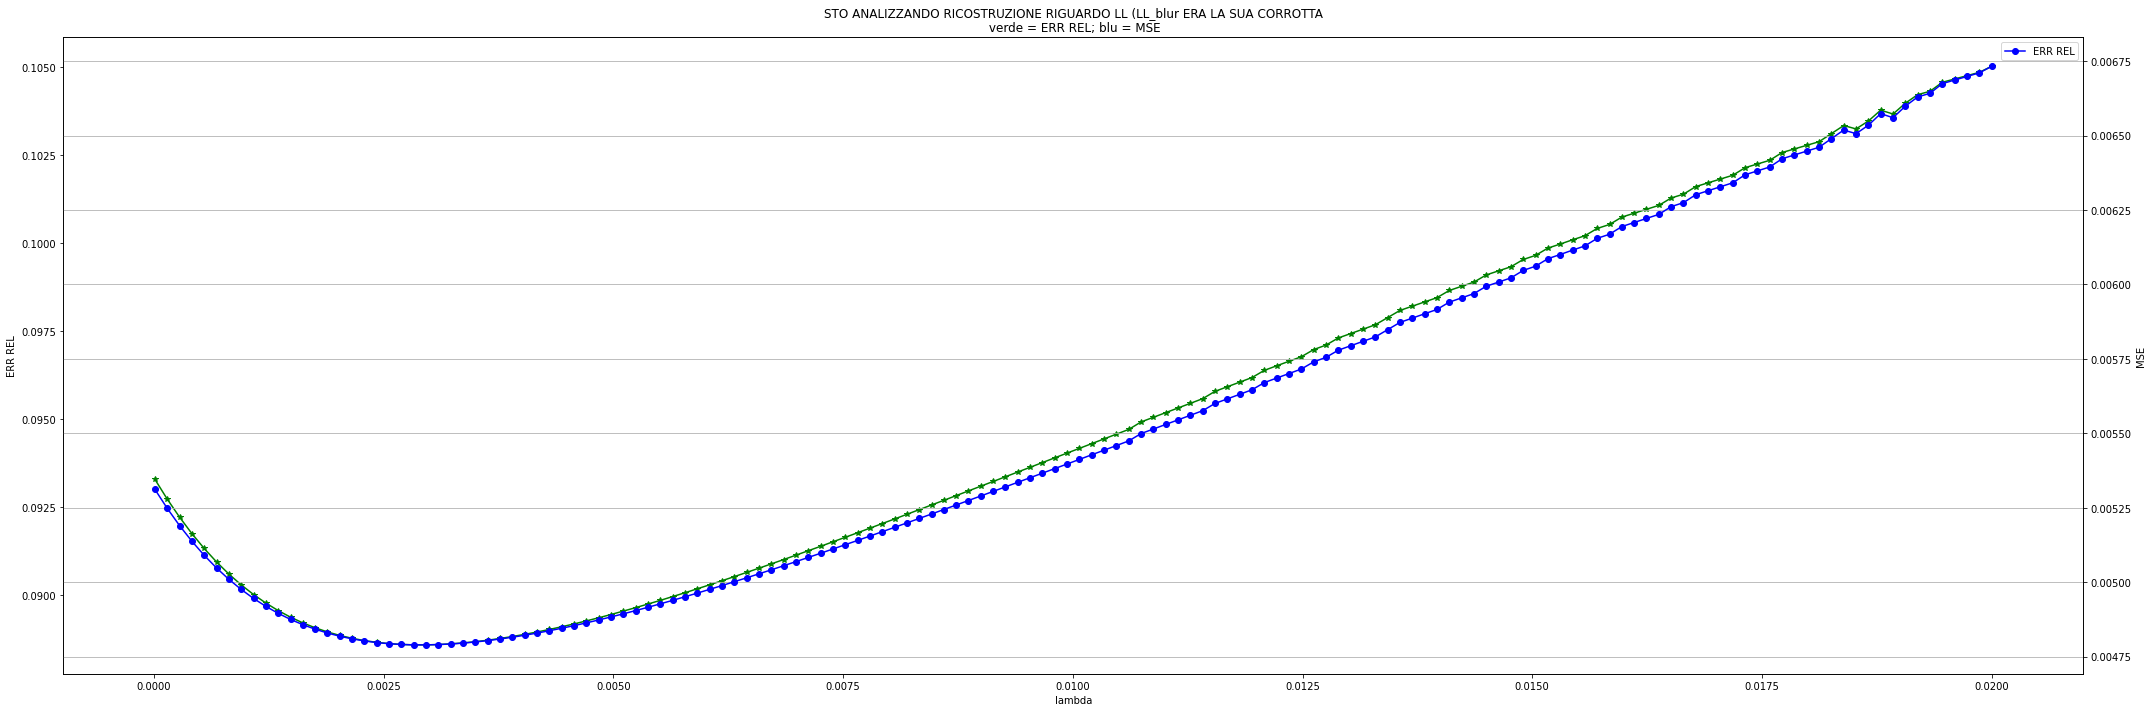
\includegraphics[width=0.8\textwidth]{IMMAGINI_RELAZIONE/graficoGiornaleTOTVAR_ERRREL&MSE.png}
    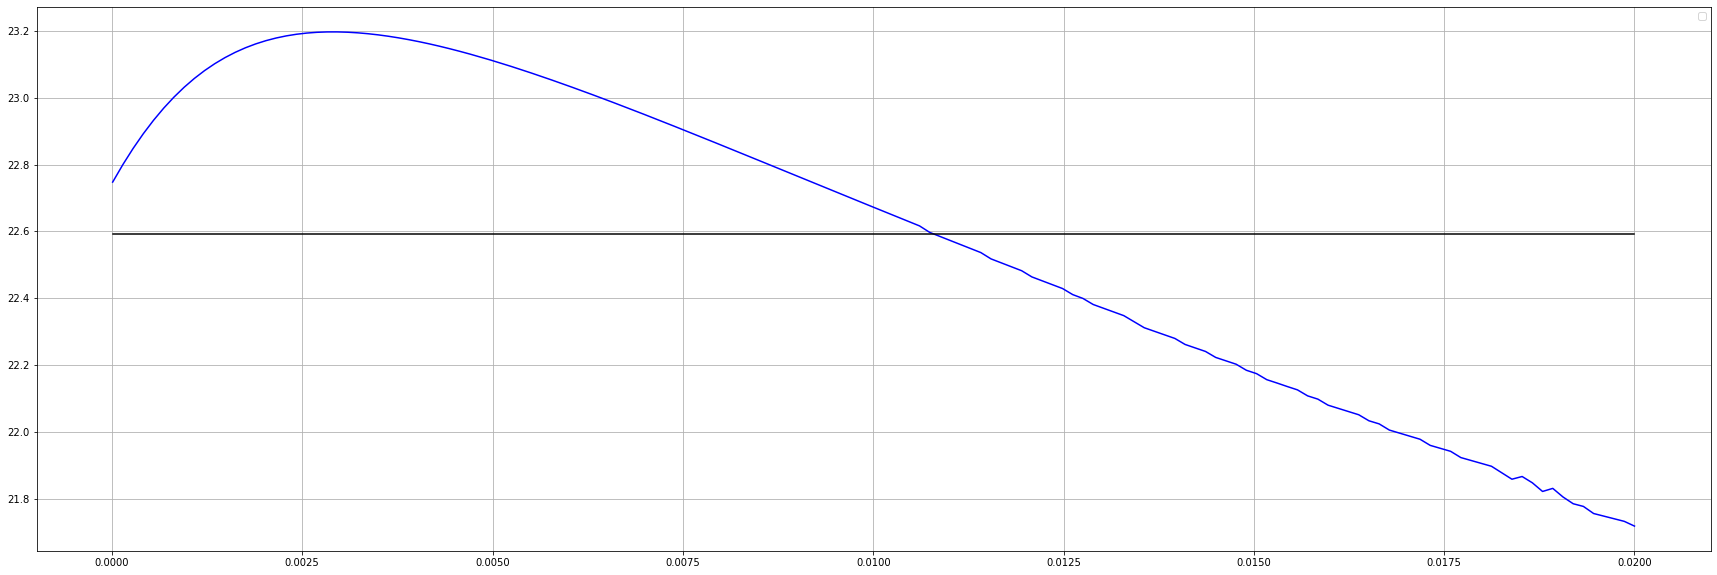
\includegraphics[width=0.8\textwidth]{IMMAGINI_RELAZIONE/graficoGiornaleTOTVAR_PSNR&suaMedia.png}
    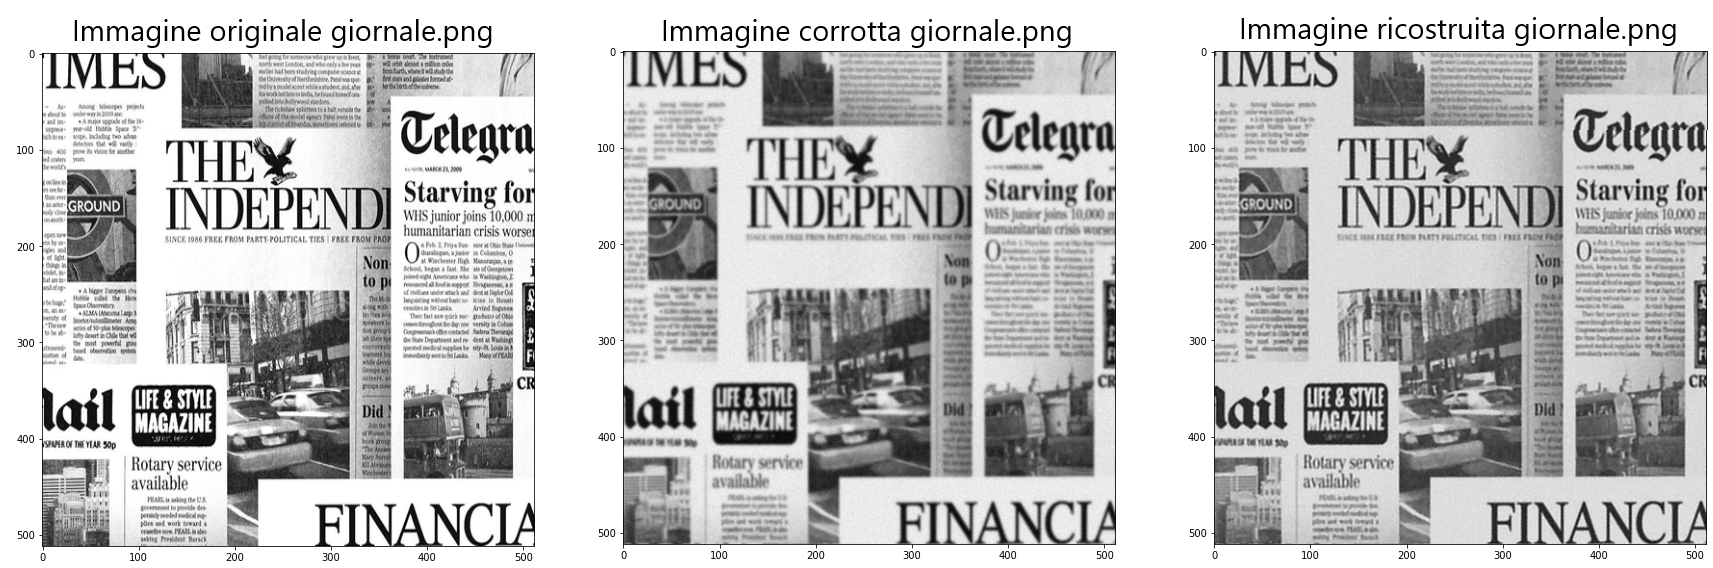
\includegraphics[width=0.8\textwidth]{imgRicostruzione/ricostruzioneGiornale_TOTVAR_maxPSNR23.20.png}
    \caption{Immagine Originale, Immagine Corrotta, Immagine Ricostruita}
\end{figure}


{\color{rred}\subsection{Variazione totale dell'immagine con testo e immagini:}}
\begin{figure}[H]{}
    \centering
    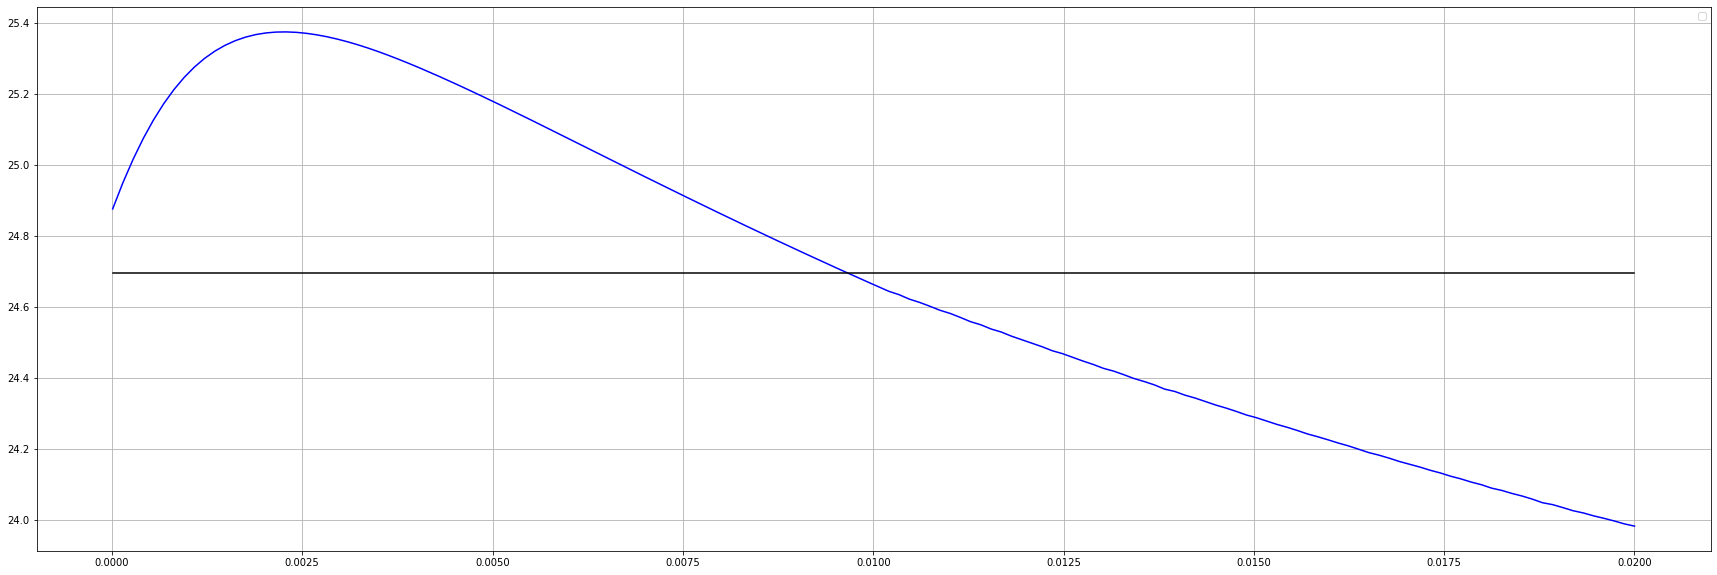
\includegraphics[width=0.8\textwidth]{IMMAGINI_RELAZIONE/graficoAlbumTOTVAR_ERRREL&MSE.png}
    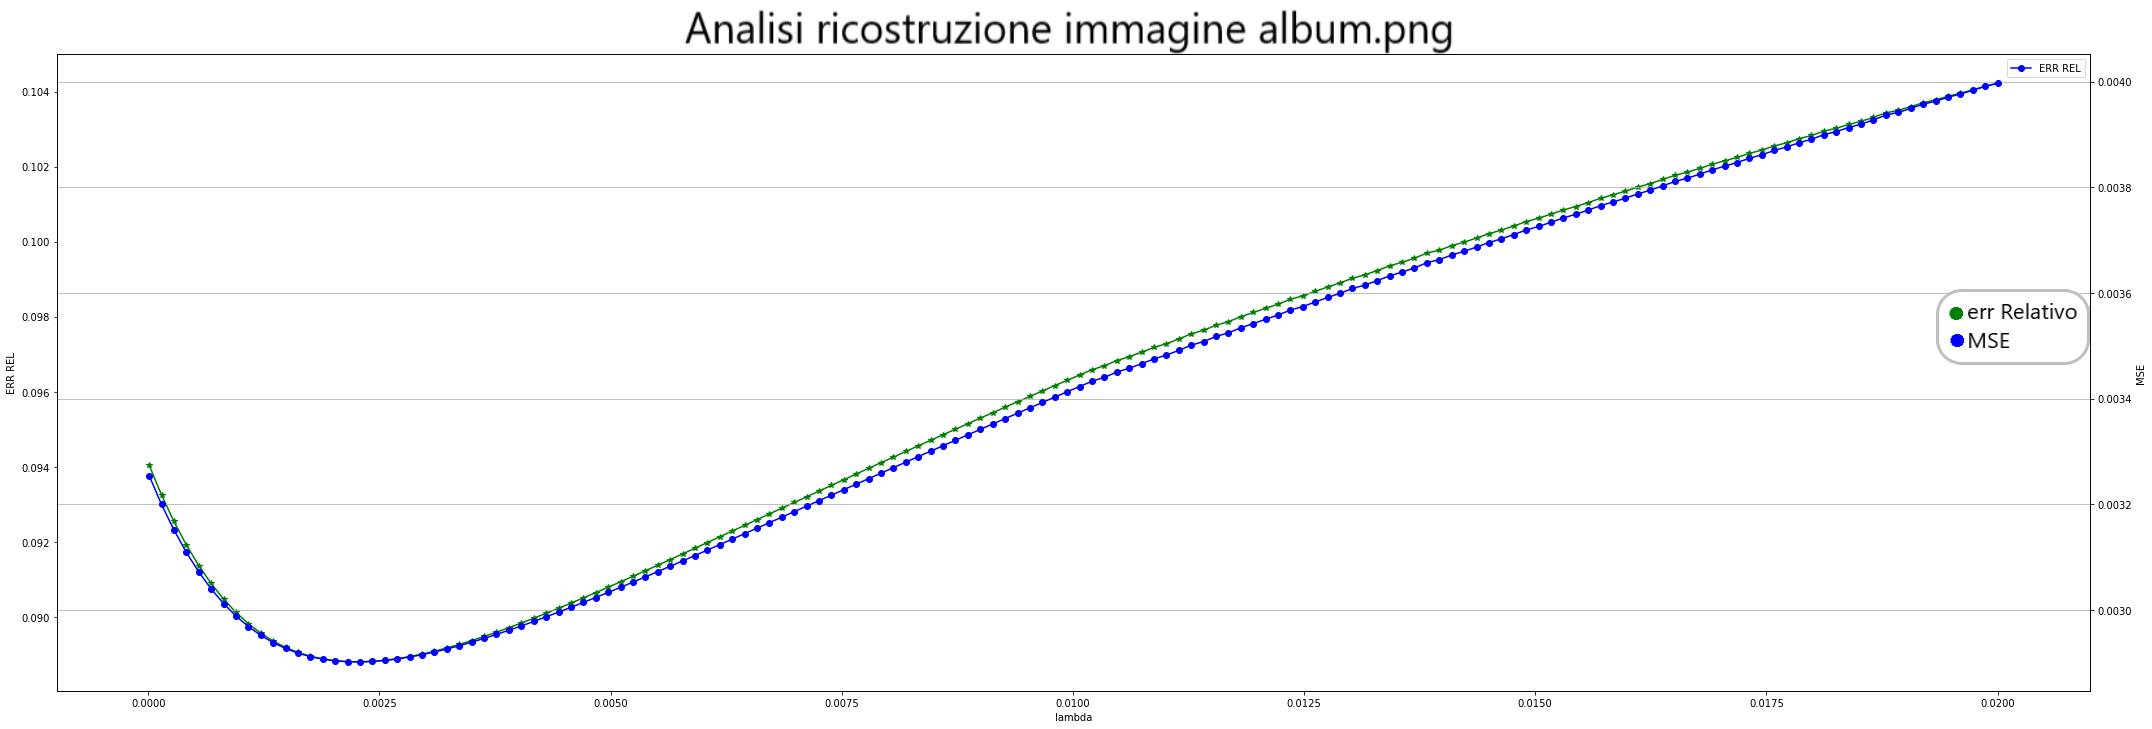
\includegraphics[width=0.8\textwidth]{IMMAGINI_RELAZIONE/graficoAlbumTOTVAR_PSNR&suaMedia.png}
    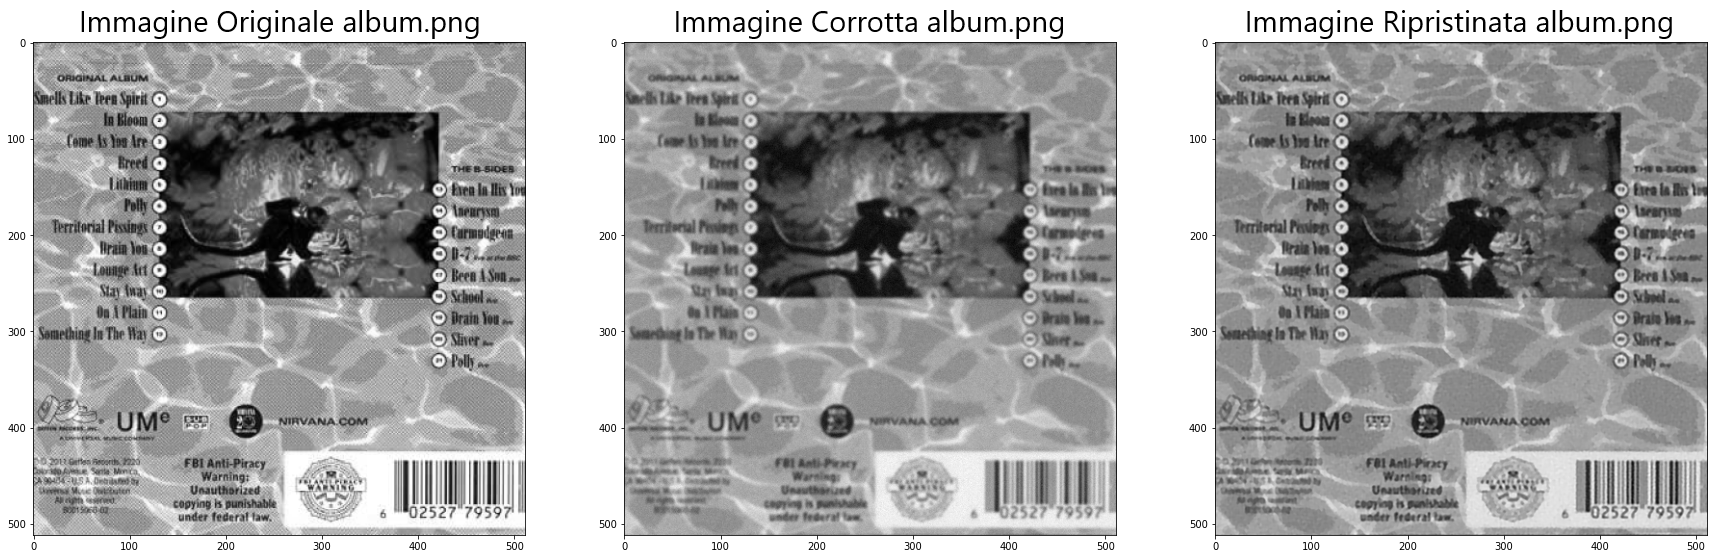
\includegraphics[width=0.8\textwidth]{IMMAGINI_RELAZIONE/eventuale_ricostruzioneTOTVAR_Album_33.71.png}
    \caption{Immagine Originale, Immagine Corrotta, Immagine Ricostruita}
\end{figure}
